
\chapter{Related Work}
\label{chap:related_work}
This chapter situates the present work within the broader literature on molecular representation learning and property prediction. We broadly review the development of graph representation learning, the classical approaches to molecular property prediction, the trade-offs between end-to-end and hybrid modelling strategies, and the specific challenges of model evaluation under data scarcity. A more formal discussion of models mentioned in this chapter is left to Chapter~\ref{chap:math_foundations}.

\section{Graph Representation Learning for Molecular Data}

\subsection{Message Passing and the D-MPNN}
The application of deep learning to molecular data has been driven by the Message Passing Neural Network (MPNN) framework, formalized by Gilmer \textit{et al.}~\cite{gilmer2017neural}. This framework unifies earlier atom-centric approaches~\cite{duvenaud2015convolutional, kearnes2016molecular} by treating representation learning as an iterative process of local information aggregation. While early models demonstrated that neural networks could learn chemically meaningful features directly from structure, their effective depth was limited. As network depth, i.e. the number of message passing steps, increases, standard MPNNs become prone to ``oversmoothing'', a phenomenon formalized by Li \textit{et al.}~\cite{li2018deeper} wherein repeated aggregations cause node representations to exponentially converge to indistinguishable vectors. 
This degradation is exacerbated by the ``tottering'' problem, first identified in the context of molecular graph kernels (pre-GNNs) by Mahé \textit{et al.}~\cite{mahe2004extensions}. They observed that random walks on molecular graphs would frequently step back and forth along the same bond, flooding the representation with redundant local information. Dai \textit{et al.}~\cite{dai2016discriminative} later demonstrated that standard node-centric GNNs suffer from this same inefficiency, as messages continuously cycle between adjacent nodes ($u \to v \to u$).

To address these structural limitations in chemical applications, Yang \textit{et al.} introduced the Directed Message Passing Neural Network (D-MPNN)~\cite{yang2019analyzing}. By operating on directed bond states rather than atom centers, the D-MPNN explicitly prevents immediate message backtracking.  This architectural choice reduces the rapid accumulation of redundant information and has empirically established the D-MPNN as a robust standard baseline for molecular property prediction.

\subsection{Expressivity and Global Context}
Xu \textit{et al.} established that standard MPNNs are limited in expressivity by the 1-dimensional Weisfeiler--Lehman (1-WL) graph isomorphism test~\cite{xu2018powerful, morris2019weisfeiler}.

The 1-WL test is a classical algorithm that determines whether two graphs are topologically identical by iteratively aggregating the labels of neighbouring nodes~\cite{weisfeiler1968ve}. In a chemical context, this theoretical upper bound implies that standard message-passing architectures cannot perfectly distinguish certain non-isomorphic molecules, such as highly symmetric cyclic structures or specific structural isomers, regardless of network depth or parameterization.

While architectures like the Graph Isomorphism Network (GIN) were developed to provably achieve this maximum 1-WL expressivity~\cite{xu2018powerful}, overcoming the 1-WL limit entirely requires fundamentally different approaches. To distinguish non-isomorphic graphs that 1-WL cannot, higher-order GNNs and subgraph-based methods have been proposed~\cite{morris2019weisfeiler, bodnar2021weisfeiler}. Additionally, to capture long-range node interactions that local message passing struggles to model, attention mechanisms and transformer-based architectures originally developed for natural language processing~\cite{vaswani2017attention} have been adapted to the graph domain. These include Graph Attention Networks (GATs)~\cite{velivckovic2017graph} and transformer-style models such as Graphormer~\cite{ying2021transformers}. However, increased theoretical expressivity often comes at the cost of statistical efficiency. Empirical benchmarking suggests that these complex, computation-heavy architectures rarely outperform simpler message-passing schemes on the small, noisy datasets typical of experimental chemistry~\cite{rampavsek2022recipe}. This gap highlights the practical preference for relatively simpler architectures, such as the D-MPNN, in low-data regimes.

\section{Predictive Modelling Paradigms}

\subsection{Classical vs.\ Neural Approaches}

Before the widespread adoption of GNNs, molecular property prediction was typically framed as a supervised learning problem on \emph{fixed} molecular representations and hand-crafted descriptors, paired with classical regression algorithms such as Random Forests and gradient-boosted decision trees (e.g., XGBoost)~\cite{breiman2001random, friedman2001greedy, chen2016xgboost}. A widely used family of fixed representations is the \emph{Extended-Connectivity Fingerprint} (ECFP)~\cite{rogers2010extended}, also known as the Morgan fingerprint. 

Morgan fingerprints represent a molecule as a binary vector encoding the presence of local substructures. Starting from atom-centered identifiers, neighbourhoods are iteratively expanded out to a specified radius (measured in bond hops), producing a multiset of hashed substructure identifiers. These identifiers are then folded into a fixed-length bit vector of dimension $d$ (e.g., $d=2048$), where each bit indicates the presence of at least one corresponding substructure. In this work, we refer to Morgan fingerprints by their radius and bit-length (e.g., radius 2, 2048 bits).

Classical models were also commonly trained on physicochemical descriptors (e.g., molecular weight, topological polar surface area)~\cite{mauri2020alvadesc} and, in some settings, features derived from quantum-chemical simulations. In particular, time-dependent density functional theory (TD-DFT)~\cite{casida1995time} provides physically grounded estimates of excited-state quantities such as vertical excitation energies, but its computational cost limits its applicability for large-scale screening.

These fixed-representation approaches remain competitive in many low-data regimes due to their strong inductive biases and statistical efficiency, and because tree-based models are often robust to irrelevant or noisy features~\cite{grinsztajn2022tree}. In contrast, end-to-end neural models learn both the molecular representation and the predictor jointly from data~\cite{wu2018moleculenet}. While this can enable the model to capture complex, task-specific structure--property relationships~\cite{ju2021machine}, it also couples representation learning and regression in a single optimization problem. As a result, end-to-end models can be sensitive to initialization and training stochasticity, leading to higher variance in predictive performance across random seeds~\cite{chuang2020debiased}.

\subsection{Hybrid and Decoupled Strategies}
Hybrid modelling attempts to combine the representational power of GNNs with the robust inference of classical regressors. By decoupling representation learning from prediction, the neural encoder can be used to map discrete molecular graphs into a continuous latent space, which then serves as input features for a downstream model. Deng \textit{et al.} introduced \textit{XGraphBoost}, where they showed that extracting the learned molecular representations from a trained GNN and feeding them into a downstream XGBoost regressor improves upon end-to-end performance across an array of benchmarks~\cite{deng2021xgraphboost}.
While common in general machine learning (e.g., ``frozen encoders'' or ``linear probing''), this strategy is underexplored in molecular machine learning as a mechanism for improving prediction under data scarcity.

\section{Learning Under Scarcity and Distribution Shift}

\subsection{The Limits of Pretraining}
In natural language processing and computer vision domains, a common strategy to mitigate data scarcity is pretraining on large supervised or unsupervised corpora, and allowing the model to adapt to the nuances of the dataset of interest through fine-tuning~\cite{devlin2019bert}. However, the transferability of molecular representations is highly conditional~\cite{you2020graph, qiu2020gcc}. Hu \textit{et al.} show that naive transfer strategies report frequent ``negative transfer'', where features learned on a source task degrade performance on a target task due to domain mismatch. Even with their more complex pretraining strategies developed specifically for molecular graphs, they often observe no benefit for regression tasks~\cite{hu2019strategies}. Furthermore, fine-tuning pretrained models reintroduces optimization challenges, with performance often depending more on the fine-tuning protocol (e.g., learning rates, freezing schedules) than the pretraining objective itself~\cite{mosbach2020stability}.

\subsection{Model Stability and Evaluation}

Given the heterogeneity of optical property datasets, standard evaluation metrics based solely on mean predictive accuracy can obscure model reliability. In molecular machine learning, performance is often dominated by the choice of data splitting strategy, particularly under scaffold-based splits that explicitly enforce distribution shift~\cite{wu2018moleculenet}. 

\begin{figure}
  \centering
  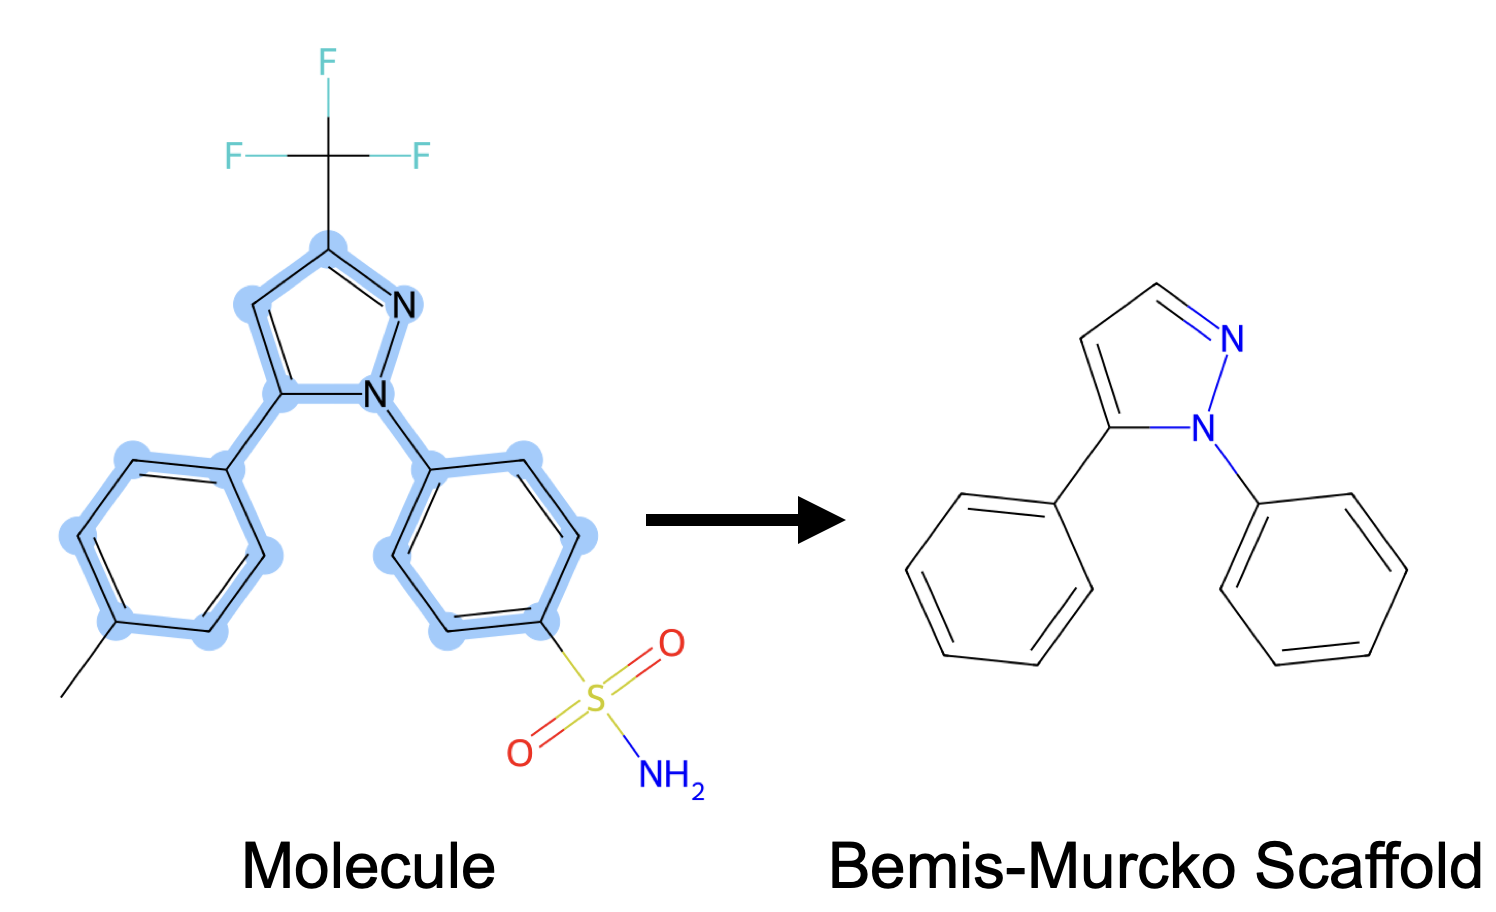
\includegraphics[width=0.6\linewidth]{Images/bemis_murcko_figure.png}
  \caption{\textbf{Depiction of a molecule and its corresponding Bemis--Murcko scaffold.} The left image shows the molecule, and the right image depicts the Bemis--Murcko scaffold representation.}
  \label{fig:bemis}
\end{figure}

A widely used scaffold split is based on Bemis--Murcko scaffolds~\cite{bemis1996properties}, which define the \emph{core framework} of a molecule by retaining ring systems and the linkers connecting them while removing peripheral substituents, depicted in Figure~\ref{fig:bemis}. Molecules are grouped according to this scaffold, and the resulting groups are then assigned to training, validation, and test sets such that scaffolds do not overlap across splits~\cite{wu2018moleculenet}. In contrast to random splits, this protocol prevents the model from benefiting from near-duplicate analogs across sets and more closely reflects the intended use case of molecular screening: predicting properties for new chemical families rather than minor variants of known structures.